
\documentclass[10pt]{report}

\usepackage{geometry}
\geometry{
  a4paper,
  textwidth=7cm,
  left=40mm,
  right=25mm,
  top=25mm,
  bottom=25mm,
  }
\usepackage[utf8]{inputenc}
\usepackage{cite}
\usepackage{url}
\usepackage{dsfont}
\usepackage{graphicx}
\graphicspath{{images/}}
\usepackage{mathtools}
\usepackage{amsmath}

\setlength{\parindent}{0em}
\setlength{\parskip}{1em}


\usepackage{chngcntr}
\counterwithout{figure}{chapter}

\usepackage{titlesec}
\titleformat{\chapter}[display]
{\normalfont\huge\bfseries}{\chaptertitlename\ \thechapter}{20pt}{\Huge}   
\titlespacing*{\chapter}{0pt}{-50pt}{25pt}
\titlespacing*{\section}{0pt}{0pt}{0pt}
\titlespacing*{\subsection}{0pt}{0pt}{0pt}
\title{Analysing Narratives: Automatic Descriptive Feature Extraction Through Latent Entity modelling}
\author{Adam Slack}
\date{}

\begin{document}

 
\begin{titlepage}
  \maketitle
\end{titlepage}

% TABLE OF CONTENTS - SPACING CHANGE, TOC, SPACING CHANGE
\renewcommand{\baselinestretch}{0.5}\normalsize
\tableofcontents
\listoffigures
\renewcommand{\baselinestretch}{2.0}\normalsize

%
%
% Chapter 1 - Introduction
%
%
\chapter{Introduction}

\section{Introduction}
The Web; A seemingly ever-expanding resource, with data being generated and information published at an accelerating rate~\cite{WebServer-lc}. As more gain access to the internet, the rate at which new information is made available will only increase. Whether the origins of data be, social media, news outlets, or e-commerce reviews, much of the resources on the web exist in a natural language format. From this data there exists underlying information that can be extracted and utilised in decision making process. Given the amount of processing required to consume data on this scale, it is necessary to ensure that computational methods exist that can accommodate for individual or business needs to understand data. Many methods for Methods that allow the processing of data to extract surface level information exist, however there is room for further understanding. By relating distinct pieces of information or subsets of data, it is possible to frame or contextualise a solution to a problem within a wider setting. This paper aims to provide a novel method capable of providing succinct summaries of documents in terms of entity topics.

Information Retrieval (IR), Machine Learning (ML), and Natural Language Processing (NLP) when considered in conjunction with each other,  concern themselves with the extracting of information from data in a natural language texts. Relating textual data yields information valuable to many different entities, including businesses when marketing products, individuals when choosing what to read, and even researchers considering the current state of a research area. For a business, relating entities extracted from texts, can help identify target groups to aim products at. For an individual, relating entities can assist in decisions on what to read, buy, and watch based on similarities between things that they do and don’t like. For research, the identification of common themes, or prominent authors can be achieved through the relating of entities.

A Latent Entity in this investigation is defined as an abstract representation of some entity that can be used to describe one or more concrete entities. Thus the term Latent Entity Modelling is defined as a transformation from a corpus of text to a collection of Latent Entities describing a corpus. Latent Entities represent a layer of abstraction from a corpus,  wherein it is possible to describe the corpus as a whole in terms of the Latent Entities.
Entity models build upon the concept of topic modelling, particularly the kinds of topics derived through Latent Dirichlet Allocation. A Topic in this sense is a probability distribution of words, such that the degree of membership for each word in a topic indicates the probability of that word being an indicator of that topic.


\section{Aims and Objectives}
The aims of this project are two-fold. The first aim is to utilise and extend natural language processing methods to model and extract latent information describing entities within narratives. The second aim is to develop a system within which corpora can be easily and effectively analysed and explored when methods developed for aim one are applied.

Natural Language Processing is a large field with many analytical methods available for modelling purposes, and as such the scope of the first aim is required to be well defined. Objectives for the first aim include:

\renewcommand{\baselinestretch}{1.0}\normalsize
\begin{itemize}
\item To survey the fields of Natural Language Processing and Topic Modelling to identify methods valuable for the task of Entity-Topic Modelling.
\item To Define a Entity-Topic Modelling method capable of deriving interpret-able topics which describe entities within narratives.
\end{itemize}

The second aim involves the development of a software environment, the objectives of which include:
\begin{itemize}
\item To develop a front-end user interface for the visual exploration of entity-topic models.  
\item To implement back-end infrastructure allowing for dynamic visualisations in front-end user interfaces.
  \item To create a software pipeline that extracts entity-topic data from a provided corpus.
\end{itemize}
\renewcommand{\baselinestretch}{2.0}\normalsize

\section{Motivation}
Motivations for this project include the need for more effective methods and tools capable of analysing data in natural language form. Additionally the development of tools utilising these methods can assist in providing others with means of understanding more about themselves, their habits, and their preferences.


%
%
%  Chapter 2 - Literature Review
%
%
\chapter{Literature Review}

\section{Introduction}
Natural Language Processing (NLP) is a vast field of study within Computer Science and Computational Intelligence, the focus of which is the development of intelligent systems capable of handling data in the form of natural language. The task of extracting Latent Entity Models is one that will touch upon many areas of NLP, including Part-of-Speech (POS) tagging, Named Entity Recognition (NER), and Latent Topic Modelling. Given that the focus of this paper is the extraction of descriptive information of narratives, it is necessary to consider the field of Information Retrieval and existing methods of descriptive summarisation as well.

It is possible to divide NLP into two large schools of thought; One involves the processing of natural language such that machine usable resources are available, the other is concerned with the application of information resulting from processed natural language. Whilst many NLP tasks require methods for parsing, understanding, or synthesising spoken words, this paper is only considering written texts. As such, the spoken language aspects of NLP will be overlooked.

Parsing written texts begins with tokenization. This is the division of a single string of characters in to strings representing sentences or words. Often text is tokenized into sentences, and each sentence is then tokenized into words. Once a text is expressed with basic sentence and word structure it is possible to apply additional processing steps. POS tagging is the application of tags to sequences of words, each tag and resulting sequence represents the grammatical structure of a sequence of words. NER is the extraction of entities from natural language, entities are tagged depending on their type. NER is performed after tokenization, however it doesn’t necessarily rely on text being POS tagged first.

There are a range of NLP tasks involving the applications of natural language parsing. From Customer relation Chatbots, to Document Summarisation and Relation. Whilst many applications involve the use of parsed text features, many also orient themselves around additional features. For example, tools for relating and summarising distinct documents may utilise topic models and topic modelling techniques.


\section{Part-Of-Speech Tagging}
POS Tagging, is a useful task for many NLP problems. It forms a solid platform from which many investigations can be launched. The quality of a POS tagger can make or break a study. There is a range of POS tagging methods to choose from, many the highest performing taggers employ Maximum Entropy (MaxEnt) models or Hidden Markov Models (HMM). However Rule and transformation based taggers often suffice~\cite{Brill1995-sr,Brill1992-hh,Huang2009-xb,Cutting1992-vx}. There even exists hybrid models that use probabilistic or stochastic methods in conjunction with rule sets. UCREL CLAWS tagger is an example hybrid model.~\cite{Leech1994-rh}
As long as the POS tagging tool utilised performs comparably to those in literature, labouring over the type of POS tagger that is used will not overly affect the results of this study. It might be more useful to consider the subjective merits of any POS tagging libraries that already exist.
The role POS tagging plays in this study is to produce a corpus of words that can be filtered by type. When building a model of words associated with entities and deriving topics that describe entities, words such as ‘The’, ‘To’ and ‘where’ won’t provide much information about entities within a corpus. Removing them may see an improvement in the quality of any derived models.


\subsection{POS Tagging Techiques and Tools}
The Natural Language Toolkit (NLTK) by default utilises a Maximum Entropy POS Tagger using the Penn-Treebank tagset. The main benefit to this POS tagger is its ease of use and accessibility. The performance of the MaxEnt tagger used in NLTK was reported score an accuracy of 96.64\% on all words, and 85.56\% on unknown words.~\cite{Ratnaparkhi1996-oa} However, in similar implementations, certain tags had error rates of 100\% , this was likely a result of the absence of certain features necessary to correctly tag specific parts of speech like ‘TO’ which occured 14,748 times in a study and was never correctly classified ~\cite{Malecha2010-fl}. 

By comparison, the CLAWS tagger achieved a reported 96\% accuracy, though accuracy fell to 82\% when text was not preprocessed to filter spelling variants and shakespearean english words. The challenges with POS tagging is the variance of sentence structure, as well as ambiguity that can occur within the english language. Fictional narratives like that of shakespeare frequently contribute to the open classes of words (Adjectives, Nouns, etc), meaning that there is an increased likelihood of unknown or spelling variant words. Whilst modern texts are not likely to be as creative with the english language as shakespeare, it would be naive to assume the CLAWS tagger would achieve the upper bounds for its accuracy. Estimating the performance of the CLAWS tagger on the corpora being used in this investigation makes the performance of both the CLAWS tagger and NLTK’s MaxEnt tagger roughly comparable.

In much of the literature, POS tagging techniques were evaluated using corpora oriented around a specific subject or domain, like news, or personal tweets. Using corpora limited to specific domains means that any given POS tagging method might only perform as reported in literature if the same or similar corpus is used. This project will benefit from a POS tagger that performs well on general purpose text, meaning that considering many of the tools used in literature opens a potential point of failure. As POS tagging is one of the first steps performed when processing a corpus, errors could be introduced into the system early on should the POS taggers used in literature proved to be inadequate on the chosen corpus for  this project. Additionally, the effect of literature tending to focus on domain limited corpora means that studies on the quality of general purpose cross-domain POS taggers are somewhat unreported.

\section{Named Entity Recognition}
The task of extracting a list of entities from text is a similar task to that of POS tagging. It involves parsing natural language and applying entity labels to entity words. A recent survey of the field summarised that Named Entity Recognition (NER) - the task of identifying entities and labelling them as ‘Person’, ‘Organisation’, or ‘Location’ - as being essential to many tasks of computational linguistics~\cite{Nadeau2007-tp}. Similarly to POS tagging, ambiguity prevents NER from having a simple solution. It is not always clear which entity some text may be referring to, especially in situations where an entity is not referred to directly, or when entities are named in unusual ways.~\cite{Ratinov2009-gw} Its application in this study is to provide a set of entities from which topic models can be derived from and applied too. 

\subsection{NER Techniques}
NER can be carried out using a range of different statistical methods. HHMs can be used to classify entities as either a name (person, organisation, or location), time, or numerical quantity. HMM-based Chunk Taggers have a reported accuracy ranging from 87\% to 94\% depending on the size of the training set~\cite{Zhou2002-st}.

Similarly to POS Tagging, statistical methods based on Maximum Entropy can be applied with similar levels of accuracy as other methods~\cite{Borthwick1999-tg,Bender2003-lc}. Hybrid approach to NER have been investigated, by utilising HMM, MaxEnt and transformation-based learning, error rates were reduced by as much as 15\% when used with the english language~\cite{Tjong_Kim2003-ym}.

CRFs are a form of statistical model that is particularly useful for applying labels to sequence data, when applied to POS tagging or NER, CRF systems can attain error rates as low as 5.55\% and 15.96\% respectively~\cite{Lafferty2001-ab,McCallum2003-yu}.

 It is worth noting that the drawbacks that applied to publications regarding POS tagging, also apply to studies on NER. Notably, NER methods typically only concern themselves with labelling words in text, and provide no means of extracting additional information about a recognised named entity. Drawbacks common though many of the techniques revolve around the resolution of which entities are actually the same. Entities within books can be referred to directly, or indirectly, and even be addressed with different names. 

 \subsection{NER Tools}
 Many free NER tools exist on the web, including Stanford NER, Illinois NER, OpenCalais NER, and Alias-i LingPipe. In a comparison between the relative performances of these tools to classify entity types (Person, Location, Organisation) the Stanford NER achieved the second highest precision and the highest recall rates.~\cite{Atdag2013-qo}. In separate comparison of NER tagging tools, more mixed results were received for the stanford NER tool. It performed comparably generalised NER tools found in the NLTK and apache OpenNLP toolkits. On specialised datasets, specialised NER taggers tuned to the task at hand predictably outperformed an untuned implementations of the Stanford NER.
 
Focusing on the Stanford NER~\cite{Finkel2005-uz} an NER tool that utilises conditional random fields (CRF). A Java implementation, the tool exists as part of a larger CoreNLP toolkit created at Stanford University. The self-reported performance of the tool ranges from 92.15\% to 85.6\% and 92.39\% to 85.53\% for precision and recall respectively. The upper bounds for possible precision and recall relied on additional processing for handling specific features of text.~\cite{noauthor_undated-ik}. Additionally, these results are from tests occuring in 2006. Recent advances in CRFs have been utilised in subsequent versions of the Stanford NER.

\section{Topic Models}
Topic models are a way of representing a corpus of text in terms of latent or abstract topics. A topic is defined as the degrees of membership each term in a collection has to a topic. In methods like Latent Dirichlet Allocation, a corpus is expressed as a probability distribution of topics, which in turn are expressed as a probability distribution of words. Describing a specific element of a corpus in terms of topic models requires matching terms in the text to terms in the various topics, after the derivation of a set of models. 

Deriving topics from a corpus is commonly done through statistical techniques such as  Latent Dirichlet Allocation (LDA), Hierarchical LDA, Latent Semantic Indexing (LSI), or Probabilistic LSI (pLSI). However, many existing methods are in fact built upon the ideas used in LSA, for example, the valuable LDA method arose out of the shortcomings of the comparatively simple LSI ~\cite{Blei2003-dj}.


\subsection{Latent Semantic Analysis}
Sometimes referred to as LSI, Latent Semantic Analysis (LSA) is a technique that provides vector representations of documents in a corpus. These vector representations allow for quantitative comparisons of different documents. The implementation of the technique is oriented around Single Value Decomposition (SVD), and attempts to model terms in a document as being averages of the document passages which in which it occurs~\cite{Deerwester1989-yl}. Additionally, for NLP tasks It is possible to view LSA as an extension of the term frequency-inverse document frequency (tf-idf) method, this is due to the method producing a subset of the reduction carried out by tf-idf such that term occurrences with the most variation between documents are retained~\cite{Landauer1998-kx}.
The obvious shortcoming of LSA is focused purely on documents at a word level. It bears no notion of topics or themes through which documents can be related. It is possible to apply additional post processing on the output of LDA. Additionally, for this study the method is totally inadequate for the analysis of entities within the documents. The possible use of the method with regards to the automatic extraction of Latent Entity Models could relate to the extraction of entity-term associations. It has been reported that the method performs well with highly dimensional data, and comparably better than standard vector space models like tf-idf.~\cite{Kumar2004-da} As such, LSA would likely be useful as nothing more Principal Component Analysis style reduction.

\subsection{Probabilistic Latent Semantic Indexing}
Probabilistic LSA (pLSA) is derived as an effort to mathematically formalise the the ideas patented by Deerwester et. al. The formal statistical nature of the method means that the method can be used in conjunction with other models in a more predictable manner. The probabilistic approach changes the meaning of output produced by pLSA, resulting in models which numerically relate terms to some latent variable. 
When used in tasks of prediction, pLSA models outperformed models produced by LSA. pLSA, reducing the perplexity of any produced models. Notably, there is a greater difference in performance on more general purpose information retrieval tasks, than on restricted corpora.~\cite{Hofmann1999-qb}. This is likely due to the effect that sparsity has on the ability of each method. Whilst still worse than pLSA, LSA actually performed better as the sparsity of training data reduced whereas pLSA’s performance decreased. This suggests that the mixture models used in pLSA perhaps overfit as the sparsity of data decreases.
As this study is focused on written narratives, any corpora used will be diverse and intrinsically sparse. As such the overfitting problem potentially reducing the effectiveness of pLSA might not be so much of an issue. However, whilst it does begin to numerically relate variables, there is still no explicit relation between documents expressed within the models meaning that adding additional documents to the corpus would mean the algorithm needs to be re-run, Additionally, there remains no direct means of relating entities or expressing entities in terms of elements within a corpus.

\subsection{Latent Dirichlet Allocation}
Latent Dirichlet Allocation (LDA) uses mixture models to generate a collection of topics which can be used to describe individual documents within a corpus. By representing individual topics as probability distributions of words found within the corpus, additional documents can be expressed as distributions of the topics already derived. This approach overcomes some of the drawbacks of the pLSA method, whilst providing a somewhat human-interpretable representation of the corpus.~\cite{Blei2003-dj}

{\hspace*{40mm}Needs reworking...}

For each document win a corpus \(D\), LDA produces a mixture model representing  \(k\) topics for \(w\). Where each word \(w_n\) of length \(N\), has a set denoting the probability of \(w_n\) belonging to each of \(k\) topics. Collections of models could be compared conceptually to weighted groups produced by some clustering method.

\renewcommand{\baselinestretch}{1.5}\normalsize
The simplified process for generating an LDA model across \(m\) documents is as follows:

\renewcommand{\baselinestretch}{1.0}\normalsize
\(1. Choose\, N \sim Poisson(\xi)\)\\
\(2. Choose\, \theta_m \sim Dirichlet(\alpha)\)\\
\(3. For\, each\, of\, the\, N_m\, words\, w_{m,n}:\)\\
{\hspace*{15mm} \(a)\, Choose\, a\, topic\, z_{m,n} \sim Multinomial(\theta_m)  \)}\\
{\hspace*{15mm} \(b)\, Choose\, a\, word\, w_{m,n} \sim Multinomial(\phi_{z_{m,n}}) \)}\\

\begin{figure}[h]
  \caption{LDA Plate Notation\label{fig:lda_plate_notation}}}
\end{figure}
\renewcommand{\baselinestretch}{2.0}\normalsize

\renewcommand{\baselinestretch}{1.0}\normalsize
The total probability of an LDA model is defined as:

\[
  P(\underline{W},\underline{Z},\underline{\theta},\phi|\alpha,\beta) = \prod P(\phi_i|\beta) \prod P(\theta_j|\alpha)\prod P(Z_{j,t} | \theta_j)P(W_{j,t} | \phi_{z_{j,t}})
\]

\renewcommand{\baselinestretch}{2.0}\normalsize
In LDA, the lengths of documents are said to be Poisson distributed, and that the set of probabilities  generated for each word wnis a random multinomial dirichlet distribution. There is little reasoning for these assumptions. The use of Poisson distributions in literature seems to be a standard distribution for estimating document lengths. However, given that the lengths of documents are known parameters, the first step in the process is redundant leaving only steps 2 and 3.

The versatility of LDA is one of its strongest characteristics. The method has seen use in a range of different settings, from filtering web spam, to the semantic annotation of satellite images. As a bayesian statistical process, it is possible to utilise other methods with relative ease given its modularity.

In web spam filtering, LDA has been combined with tf-idf and expanded to take into consideration links that exist between documents. For spam classification, the use of LDA as a bayesian network performed worse than baseline machine learning methods, however improvements were seen when the method was expanded and combined with other statistical techniques.~\cite{Biro2008-ld}

For automatic image annotation, additional machine learning and computer vision methods can be applied to images in order transform images into collections of image features. Topics derived from a corpus of these images can be used to annotate new images introduced. Attempts at using LDA in image annotation have seen some success, whilst not all annotations from topics were correct, they were often at least conceptually related.~\cite{Feng2010-dp, Zhang2011-dn}

LDA doesn’t relate words semantically. The meanings of words in a topic are not necessarily relate in any way, which is demonstrated in studies using LDA to annotate images. This means that derived topics might not provide any meaningful grouping of words. The intuition is that words in books and documents about a specific subject will somewhat relate to other words in the document. LDA might not produce thematically related topics if the documents used to derive topic distributions are varied in content. For this investigation, the potential for thematically unrelated topics is potentially a major drawback. Entities within narratives might be present throughout a whole series of books. Meaning that they may be associated with a wide range of topics. It is unclear at this stage what effect this may have on the quality of derived topics. It might be necessary to regard the same entity across two books to actually be distinct.

As a bag of words method, each unigram is treated as being unrelated to other words. Which is not true in the case of written narratives. Much of the meaning of words and relations between words are lost when used in ‘bag of word’ models. The drawback for this study is that relations between terms and entities are required. If topics were directly derived from the documents which entities were extracted from, then there would be no meaningful way of identifying how these topics apply to entities.

\section{Evaluating Topic Models}
Topic models are machine representations of word groups that have been deemed to be somehow related. The challenge for evaluating topic models is that it depends on the task which they are being applied to. Directly evaluating the accuracy of topic models is tough, as an unsupervised bayesian method, the probabilities are not interpretable, they are what they are and no ground truth exist. Where produced models can be effectively evaluated is on their efficacy at some secondary task, this could be to predict or estimate topics that might be present in documents not present in the sample used to train models.


\subsection{Perplexity}
Perplexity is a commonly used metric accross topic modelling literature, and is an estimate of how well a probability distribution or probabilistic model predicts a sample. In the literature for pLSA and LDA, perplexity is one of the main metrics used to evaluate the quality of the methods.~\cite{Blei2003-dj,Hofmann1999-qb} 

Perplexity can be calculated by subsampling a corpus into training and testing sets. By using the test set as unlablled data the perplexity of a model is measured as its ability to estimate the probabilities density of the \(M\) documents in the test set.

\renewcommand{\baselinestretch}{1.0}\normalsize
For LDA, the perplexity is defined as:

\[
  perplexity(D_{test}) = exp({-{{\sum^{M}_{d=1} log(p(w_d))}\over{\sum^{M}_{d=1} N_d}})
\]

\renewcommand{\baselinestretch}{2.0}\normalsize
The probability of a word \(w_d\) is seemingly glossed over in many papers, however some methods for estimating the value have been proposed. The harmonic mean is often used as an estimator due to its relative simplicity and computational efficiency, however it has been subject to criticism regarding its suitablity for these Other methods including 'left-to'right' and a chib-style estimator have been shown to be more effective estimators.~\cite{Newton1994-ws,Wallach2008-ti,Chib1995-wq,Wallach2009-ot}


The use of perplexity as a metric for evaluating topic models does not necessarily mean that the model is correct or accurate, but rather that the model is capable of predicting a sample, not that the prediction is correct. If a topic model assigned equal proabilities accross all words in a vocabulary, then the perplexity would be high, indicating that the topic model provides no insight into the relationships between documents.

\subsection{Interpretability and Coherence}
For human interpretable topic models, it is necessary that the terms within each topic be semantically related, or that it is clear why words in a topic co-exist. Whilst attempts have been made to utilise machine learning methods in the production of coherent topic models, the evaluation of them is somewhat lax. Whilst on the surface, models appear to be more coherent with the inclusion of methods like Markov Random Fields, the coherence is often done subjectively using the opinions of juman judges.~\cite{Xie2015-wv} Even though the use of human judges may be an imprecise method of evaluation, it does provide insight into the interpretability of derived models. For tools that aim to provide users with insight into large corpora of data, interpretability of the results is a key element defining the success of the tool. With low coherence of topics and thus low levels of interpretability, communicating any extracted information becomes increasingly difficult.

Assessing the interpretability and coherence of topic models has been somewhat formalised through the proposal of a ‘word intrusion’ and ‘topic intrusion’ tests. The word intrusion test assesses the coherence of a topic by introducing words that don’t belong in a topic and asking humans to identify the misplaced word. A Topic Intrusion test is performed by introducing an incorrect topic and asking humans to identify the misplaced topic. It was found that in cases where topics are incoherent or difficult to interpret, that humans would tend to choose a word seemingly at random.~\cite{Chang2009-jr}. This method has been extended by asking humans to select two intruder words, where only one of them is actually an intrusion. The idea is that in well defined topics not only will the correct intruding word be selected, but also there will be no means for individuals to distinguish between the strength of belonging for the remaining words. If participants can't decide on what is an intruding word, then there should be a seemingly randomised selection.~\cite{Morstatter2016-co} Both approaches result in different assessments of any derived topics, there is no indication however as to which metric is a better estimate of the coherence of topics.

The precision metrics defined for word and topic intrusion tests may be of value when evaluating the quality of derived Entity Models, though they rely heavily on human evaluation of topics. Use of judges is time consuming and potentially unreliable. A more formal method of evaluating coherence was proposed by comparing word vectors formed in a semantic space built from wikipedia articles. By considering the distributional similarity of word vectors formed by pairs of words in topics, the semantic cohesion of topics can be estimated using one of a few different metrics. When considering the inter-rater agreement between the calculations and human raters, the spearmann rank correllation values had an average of  \(\bar{x}=0.77\) and a standard deviation of\(,\sigma=0.04\). The relative aggreement between each method of evaluation suggests that any of them could serve as valuable means of evaluating the coherence of topics. ~\cite{Aletras2013-oo}

Given a topic \(T = {w_1,...,w_n}\), the coherence of that topic is defined as the mean similarity of each possible word pairing \(Sim(w_i, w_j)\) where \(w_i, w_j \in T\). The similarity of two words could be one of many measures, including the cosine of the word vectors, or the jaccard coefficient.~\cite{Newman2010-op}

% NOTE: {n \choose m} is a combinatorics expression for the total number of possible of m pairings in a set of n elements 

\[
  Coherence_{sim}(T)=\frac{\underset{i+1<j<n}{\underset{1<i<n-1}{\sum}}Sim(w_i, w_j)}{{n \choose 2}}
\]

 
%The precision of a topic \(k\) is defined as the number of correctly identified intruding word over the total number of intruding words. 
%
%$$P_{k}^{m} = \sum_{s} \mathds{1}(i_{k,s}^{m} = \omega_{k}^{m})/S$$


\subsection{Comparing Models}
When evaluating topic models, it is often done from the perspective selecting the best topic model. This could be doen through the use of interpretability and coherence tests, or it could be done through a models performance at some secondary task.For exploratory purposes, visual means of comparison could also be used to explore the differences between models and methods.

When regarding topics as a \(k-dimensional\) model, visualising the topic space can be challenging. One approach to comparing topic models is to look at the similarities between each topic in a pair of models. In the form of a bipartite graph, it is clear which topics in two models are conceptually similar. The bipartite graph in figure~\ref{fig:topic_modelling_comparisons} shows that even though two methods do have different conceptual topics, there are some topics in both that are somewhat similar. The similarities and differences between the two models are seen further if relationships between documents are plotted.The noticable difference between the two topic modelling methods made visiable in the visualisation is that LDA appears to form relations between the document clusters that LSA kept distinct.~\cite{Crossno2011-sn}

\renewcommand{\baselinestretch}{0.5}\normalsize
\begin{figure}[h]
  \begin{subfigure}
    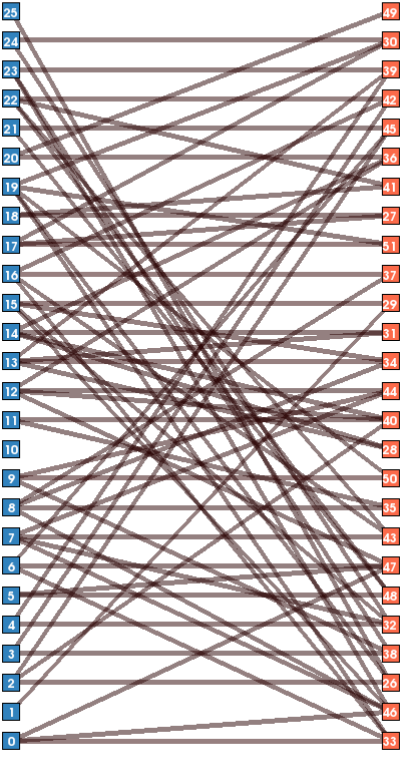
\includegraphics[scale=0.20]{lda_lsa_topic_view}
  \end{subfigure}
  \begin{subfigure}
    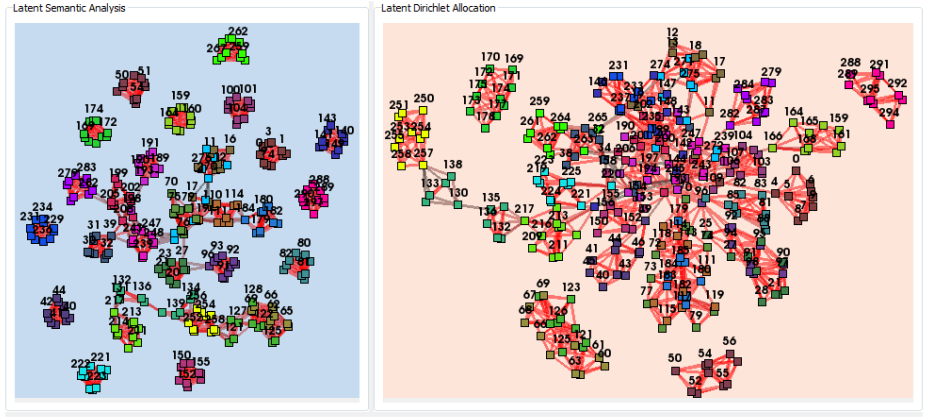
\includegraphics[scale=0.35]{lda_lsa_document_view}
  \end{subfigure}
  \caption{(Left) Bipartite topic conceptual similarity graph. (Middle, Right) Document relationships formed by LSA and LDA topic modelling methods \label{fig:topic_modelling_comparisons}}
\end{figure}

\renewcommand{\baselinestretch}{2.0}\normalsize
These visualisations might be effective at explaining why a perticular model performs in a certain way at some secondary task, or it might be useful for identifying traits of models that ar valuable for perticular tasks. However, the visualisations don't provide any quantitative insight into how one model may perform when compared to another.

\section{Entity Modeling}
Entity Modelling exists as a small field of study aside from topic modelling and could be regarded as an extention of the NER domain. It relates to the extraction of entity description s, as well as the linking of distinct entities. Many of the challenges in this field stem from the high levels of ambiguity present in natural language. Attempts have been made to utilise Topic Models in the task of entitty resolution as well as forming links and relationships between entities within a document, Whilst semantic resources have been investigated as tools for the automatic tagging of extracted entities.

\subsection{Entity Linking}
Entity linking is the task identifying how entities in a corpus relate to each other, It involves the resolution of entity mentions that refer to the same entity in order to perform optimally.

Topic models have been utilised in the task of entity linking through the application and development of specialised Entity-Topic Models.One such investigation involved finding mentions of concrete entities, such as \('iPod',\, 'Steve Jobs',\) and \(iPhone\) and forming a unifying \('Apple\, Inc'\) topic.~\cite{Han2012-gy} The approach added an additional step to the generative LDA algorithm which sampled topic, and entity assignments for each entity. The focus of the paper utilising the topical context within which each entity was mentioned, to try and resolve entities with multiple mentions through relationships that may form between entities in the model.

The Entity-Topic Models suggested are statistically sound, and perform well in predictive tasks oriented around wikipedia information. The key drawback for this study is the use of short documents to train, test, and evaluate derived models. Models were trained dataset of news articles from the TAC 2009 dataset ~\cite{Macnamee-pd}, which being short in length often benefit the assumption made in the study regarding how entities relate to the topics within the document. For longer texts and perticularly narratives, this assumption is not necessarily valid; wide ranges of topics may be present, with entities only being expressed in the context of some of these topics. The limitation of this entity-topic modelling method could come from the base LDA method. As a bag-of-words approach, 

\subsection{Entity Topic Models}



%
%
% Chapter 3 - New Ideas
%
%
\chapter{New Ideas}
\section{Introduction}
In chapter 2 many different topic modelling and wider NLP techniques were considered, with only those specific to entity-topic modelling being close to meeting the aims that this project has. The LDA Topic modelling method provides a base statistical method from which this investigation can be launched.

The main drawback with specific entity-topic modelling methods relate to the assumptions made regarding the relationships between entities and topics in a document. Not necessarily applicable to larger documents and written narratives it is clear that some adaptation is required for general LDA based entity-topic modelling methods. Additionally, there is clearly no publically available tools that allow non-technical individuals to explore and investigate entity-topic models, resulting in the field remaining relevant only in literature.

An obvious adaptation to entity-topic modelling methods is to incorporate some weighting metric to associated terms and topics, there is potential for this step to be done as a pre-processing method.

\section{Gaussian Entity-Term Matrix}

The Gaussian Entity-term matrix is a means of segmenting a given document into entities and associated terms. The matrix for a given document consists of strengths of associactions between a entity-word pairing. It functions under an assumption that the more seperation there is between two words in a document, the weaker the association is between those two words. By modelling documents not as a bag of words, but as sequences it is possible to capture some of the relationships between different words prior to applying additional statistical methods.

Given a set of entities \(\underline{E} = \{\underline{e}_0, ..., \underline{e}_i\}\) where \(\underline{e}_i = \{e_{i,0}, ..., e_{i,m}\}\), and a set of words \(\underline{W}=\{\underline{w}_0, ..., \underline{w}_j\}}\), then a matrix \(D\) when indexed by \(i,j\) can be defined as:

\[
  D_{i,j}= \sum^{|\underline{e}_i|}_{m=0}\sum^{|\underline{w}_j|}_{n=0}\sqrt{a\over{\pi}}\cdot e^{-a\cdot(e_{i,m} - w_{j,n})}
\]

\[
  D =
  \bordermatrix{&&e_0 && e_1 &&\hdots && e_i\cr
    w_0 && D_{0,0} && D_{0,1} && \hdots && D_{0,i}\cr
    w_1 && D_{1,0} && D_{1,1} && \hdots && D_{1,i}\cr
    \vdots && \vdots && \vdots && \ddots && \vdots\cr
    w_j && D_{j,0} && D_{j,1} && \hdots && D_{j,i}
  }
  
\]


\section{Analysis Pipeline}



%
%
%
%
%
\chapter{Prototyping}
\section{Introduction}

%
%
%
%
%
\chapter{Results and Evaluation}
\section{Introduction}

%
%
%
%
%
\chapter{Conclusion}
\section{Introduction}

\renewcommand{\baselinestretch}{1.0}\normalsize
\bibliographystyle{unsrt}
\bibliography{./biblio}
\end{document}
